\documentclass[12pt]{article}

% Packages
\usepackage[utf8]{inputenc}
\usepackage{amsmath}
\usepackage{amssymb}
\usepackage{graphicx}
\usepackage{hyperref}
\usepackage{amsthm}
\usepackage[margin=1in]{geometry}
\usepackage[numbers]{natbib}
\usepackage{listings}
\usepackage{algorithm}
\usepackage{algpseudocode}
\usepackage{tabularx}

% TikZ and diagram packages
\usepackage{tikz}
\usetikzlibrary{positioning,arrows,shapes,calc,decorations.pathreplacing}
\usepackage{forest}

% Theorem environments
\newtheorem{theorem}{Theorem}
\newtheorem{lemma}{Lemma}
\newtheorem{proposition}{Proposition}
\newtheorem{corollary}{Corollary}
\newtheorem{hypothesis}{Hypothesis}
\newtheorem{definition}{Definition}
\newtheorem{remark}{Remark}
\newtheorem{constraint}{Constraint}

% Title and author
\title{TranslationAI: Theory-Driven, Ethically Engineered Machine Translation}
\author{Author Name}
\date{\today}

\begin{document}
\maketitle
\begin{abstract}
This paper presents TranslationAI, an AI-assisted translation platform grounded in academic translation theory.
\end{abstract}

\section{A Strategy-First Architecture for AI Translation}

\subsection*{End-to-End Strategy-First Translation Pipeline}
A high-level TikZ diagram illustrating the main stages of the TranslationAI pipeline.

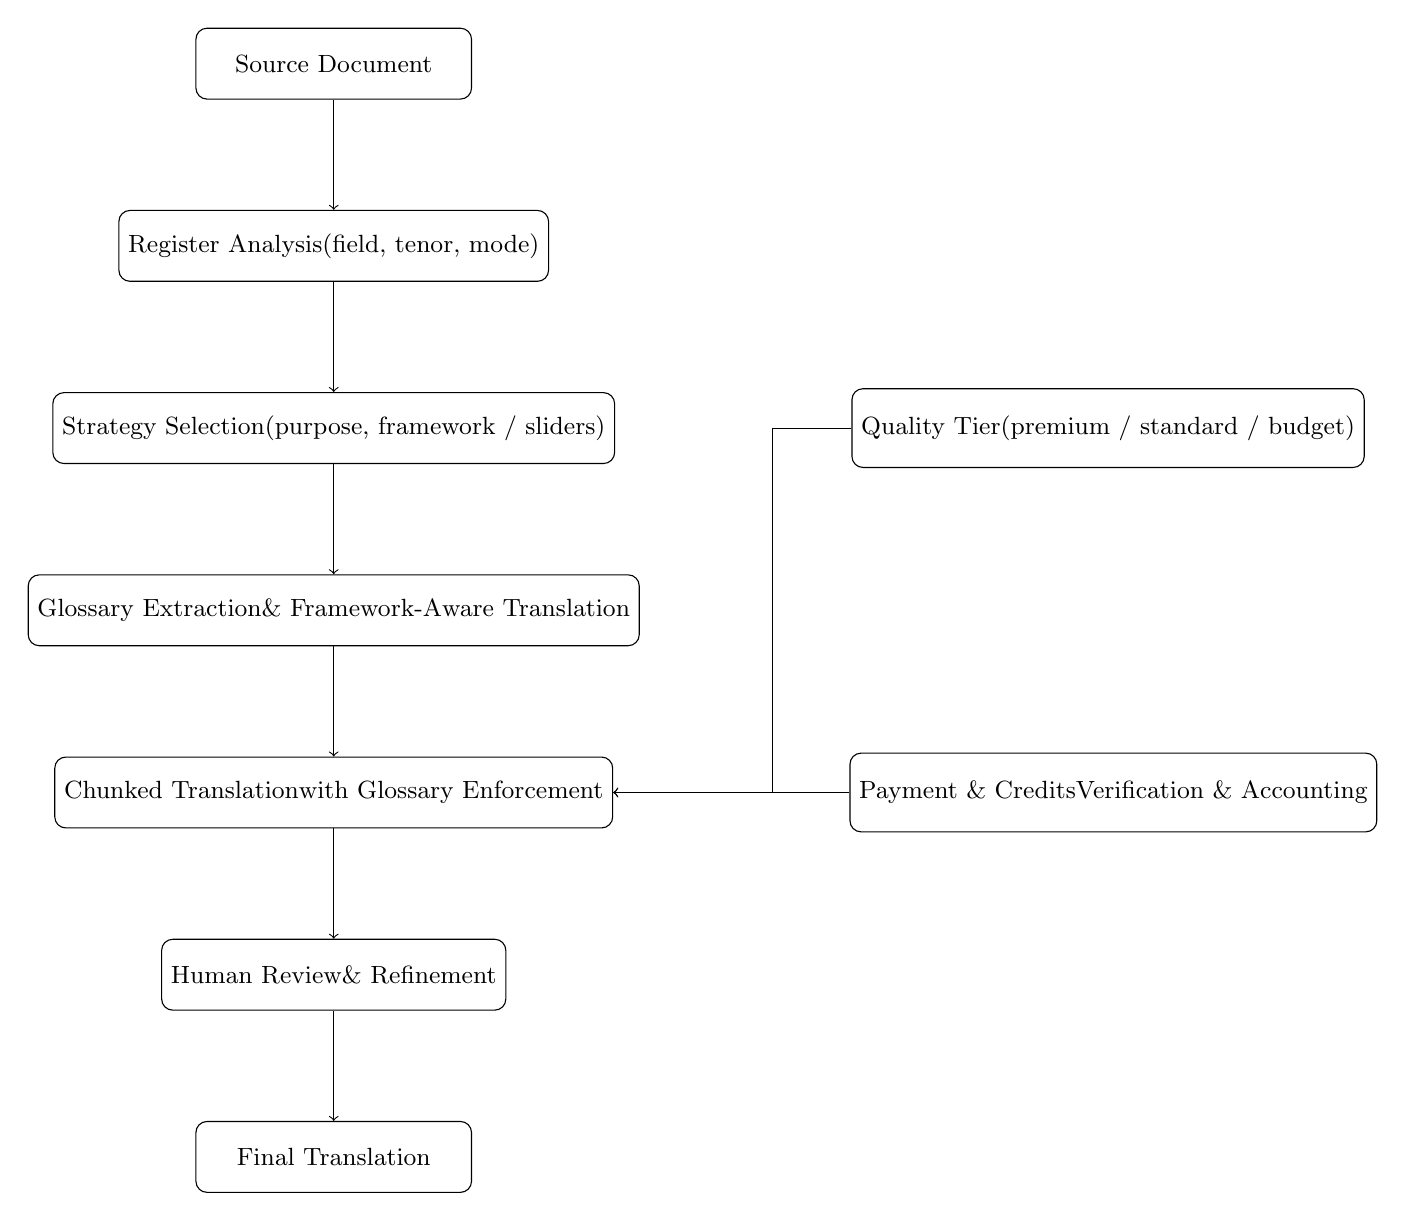
\begin{tikzpicture}[font=\small, node distance=1.4cm]
  % Nodes
  \node[draw, rectangle, rounded corners, minimum width=3.5cm, minimum height=0.9cm] (source) {Source Document};
  \node[draw, rectangle, rounded corners, below=of source, minimum width=3.5cm, minimum height=0.9cm] (analysis) {Register Analysis\\(field, tenor, mode)};
  \node[draw, rectangle, rounded corners, below=of analysis, minimum width=4.2cm, minimum height=0.9cm] (strategy) {Strategy Selection\\(purpose, framework / sliders)};
  \node[draw, rectangle, rounded corners, below=of strategy, minimum width=4.8cm, minimum height=0.9cm] (glossary) {Glossary Extraction\\\& Framework-Aware Translation};
  \node[draw, rectangle, rounded corners, below=of glossary, minimum width=4.5cm, minimum height=0.9cm] (chunks) {Chunked Translation\\with Glossary Enforcement};
  \node[draw, rectangle, rounded corners, below=of chunks, minimum width=3.8cm, minimum height=0.9cm] (human) {Human Review\\\& Refinement};
  \node[draw, rectangle, rounded corners, below=of human, minimum width=3.5cm, minimum height=0.9cm] (final) {Final Translation};

  % Arrows
  \draw[->] (source) -- (analysis);
  \draw[->] (analysis) -- (strategy);
  \draw[->] (strategy) -- (glossary);
  \draw[->] (glossary) -- (chunks);
  \draw[->] (chunks) -- (human);
  \draw[->] (human) -- (final);

  % Side node for quality tiers
  \node[draw, rectangle, rounded corners, right=3.0cm of strategy, minimum width=3.0cm, minimum height=1.0cm] (quality) {Quality Tier\\(premium / standard / budget)};
  \draw[->] (quality.west) -- ++(-1.0,0) |- (chunks.east);

  % Side node for payment and credits
  \node[draw, rectangle, rounded corners, right=3.0cm of chunks, minimum width=3.2cm, minimum height=1.0cm] (payment) {Payment \& Credits\\Verification \& Accounting};
  \draw[->] (payment.west) -- ++(-1.0,0) |- (chunks.east);
\end{tikzpicture}

\end{document}
